%%%%%%%%%%%%%%%%%%%%%%%%%%%%%%%%%%%%%%%%%%%
%%% DOCUMENT PREAMBLE %%%
\documentclass[12pt]{report}

\usepackage{agda}
\usepackage{catchfilebetweentags}

\usepackage[english]{babel}
%\usepackage{natbib}
\usepackage{url}
\usepackage[utf8x]{inputenc}
\usepackage{amsmath}
\usepackage{graphicx}
\graphicspath{{images/}}
\usepackage{parskip}
\usepackage{fancyhdr}
\usepackage{vmargin}
\setmarginsrb{3 cm}{2.5 cm}{3 cm}{2.5 cm}{1 cm}{1.5 cm}{1 cm}{1.5 cm}

\title{1}								
% Title
\author{Guilherme Horta Alvares da Silva}						
% Author
\date{15 de Abril de 2019}
% Date

\makeatletter
\let\thetitle\@title
\let\theauthor\@author
\let\thedate\@date
\makeatother

\pagestyle{fancy}
\fancyhf{}
\rhead{\theauthor}
\lhead{\thetitle}
\cfoot{\thepage}
%%%%%%%%%%%%%%%%%%%%%%%%%%%%%%%%%%%%%%%%%%%%
\begin{document}

%%%%%%%%%%%%%%%%%%%%%%%%%%%%%%%%%%%%%%%%%%%%%%%%%%%%%%%%%%%%%%%%%%%%%%%%%%%%%%%%%%%%%%%%%

\begin{titlepage}
	\centering
    \vspace*{0.5 cm}
   % 
\includegraphics[scale = 0.075]{bsulogo.png}\\[1.0 cm]	% University Logo
   \begin{center}    \textsc{\Large   Fundação Getúlio Vargas}\\[2.0 cm]	\end{center}% University Name
   \textsc{\Large Modelagem Matemática  }\\[0.5 cm]				% Course Code
	\rule{\linewidth}{0.2 mm} \\[0.4 cm]
	{ \huge \bfseries \thetitle}\\
	\rule{\linewidth}{0.2 mm} \\[1.5 cm]
	
	\begin{minipage}{0.4\textwidth}
		\begin{flushleft} \large
		%	\emph{Submitted To:}\\
		%	Name\\
          % Affiliation\\
           %contact info\\
			\end{flushleft}
			\end{minipage}~
			\begin{minipage}{0.4\textwidth}
            
			\begin{flushright} \large
        \emph{Feito por:} \\
      Guilherme Horta 
		\end{flushright}
           
	\end{minipage}\\[2 cm]
	
  \includegraphics[scale = 0.5]{FGV.png}
    
    
    
    
	
\end{titlepage}

%%%%%%%%%%%%%%%%%%%%%%%%%%%%%%%%%%%%%%%%%%%%%%%%%%%%%%%%%%%%%%%%%%%%%%%%%%%%%%%%%%%%%%%%%

\tableofcontents
\pagebreak

%%%%%%%%%%%%%%%%%%%%%%%%%%%%%%%%%%%%%%%%%%%%%%%%%%%%%%%%%%%%%%%%%%%%%%%%%%%%%%%%%%%%%%%%%
\renewcommand{\thesection}{\arabic{section}}
\section{Introdução}

Desde Novembro de 2008, o valor de mercado mundial do bitcoin chegou a 330 bilhões (em 17 de dezembro de 2018). O preço do bitcoin chegou a ter seu recorde histórico por volta de 20 mil dólares. Outras cripto-moedas também foram criadas e elas também possuem um bom valor de mercado. Cripto-moedas se tornaram instrumentos financeiros e serão as principais moedas em um futuro próximo.

Cripto-moedas também são utilizadas com contratos inteligentes. Um exemplo seria o comprador reservar uma parte do dinheiro para o vendedor na blockchain. Para o dinheiro ser liberado, o vendedor deve receber uma assinatura do comprador. O comprador irá fornecer a assinatura se o produto dele chegar. Se o produto não chegar a tempo, o comprador recebe seu dinheiro de volta. Contratos inteligentes são utilizados hoje em dia por grandes fundos, no qual as relações de contratos são integralmente governada por algoritmos (sem nenhuma interferência governamental).

\section{O bitcoin}

Já que cripto-moedas são governadas integralmente por algoritmos.
Precisamos garantir que esses algoritmos estejam corretos, uma vez que em caso de falha,
não existe nada que se possa fazer.
O único jeito de resolver problemas é criando um consenso entre usuários e mineradores,
a partir de um soft fork (retro compatível) ou um hard fork.
A possibilidade de erro é um dos maiores riscos às cripto-moedas.
Por exemplo, no protocolo inicial do bitcoin, a unicidade dos IDs das transações não era garantida.
Com isso, era possível que houvesse ataques de gasto duplo.
Isso pode ser consertado incluindo o número do bloco na transação (foi feito em um soft fork).
Outro problema do bitcoin é que o tamanho do bloco do bitcoin não é suficiente para cobrir todas as transações.
Para resolver isso, foi criada a Light Network, que é um protocolo de segunda camada do bitcoin.

Por isso, é importante a verificação completa dos protocolos criptográficos.
Um alto nível de verificação pode ser encontrado criando um método formal para cripto-moedas e provando que ele está correto.
Ainda não foi criado nenhum método completamente formal para a formalização de alguma cripto-moeda.

O crescimento de contratos inteligentes criou alguns problemas em relação a segurança de instrumentos financeiros.
O maior incidente foi a falha do DAO.
Quando o DAO chegou a um valor de 150 milhões de dólares, um usuário usou uma vulnerabilidade para hackear o contrato.
A perda do dinheiro dos investidores foi somente evitada por causa de um hard fork na rede ethereum,
no qual apagou a maioria das transações investidas no DAO.
Esse hard fork violou o principio de que o dinheiro dos usuários em cripto-moedas devem ser apenas governados por algoritmos,
sem nenhuma interferência humana.
Por isso, existe a necessidade de provas formais, que provam sua corretude e que também servem como certificado.

\section{Introdução a Agda}

Para garantir a corretude de um programa, precisamos de demonstrações formais ou técnicas de model checking.
Idealmente, deveria ser capazes de especificar e programar em uma mesma linguagem.
Agda é uma linguagem que permite isso.

Agda é um provador de teoremas baseado na teoria de tipos de Martin-Lof.
Ele está muito relacionado ao provador de teoremas Coq.
Além do mais, Agda é uma linguagem total, o que é garantido que ela sempre termina (não existe loop infinito).
Sem isso, Agda seria uma linguagem inconsistente.
Agda já está em sua segunda versão.
Ela foi criada na tese de doutorado de Ulf Norell.
Depois disso, ela foi aprimorada por sua comunidade.

Para definir-se booleans em Agda:

\ExecuteMetaData[latex/Code.tex]{bool}

Para definir os números naturais de acordo com os axiomas de peano, usa-se:

\ExecuteMetaData[latex/Code.tex]{nat}

No caso dos naturais, exite uma função sucessor. Para cada número natural, essa função retorna outro número natural.

Para definir-se soma, usa-se a definição recursiva

\ExecuteMetaData[latex/Code.tex]{plus}

Em uma lista, existe dois construtores.
Um que fornece a lista vazia e outro, que dado um elemento e outra lista, ele fornece uma nova lista.

\ExecuteMetaData[latex/Code.tex]{listdef}

Para descobrir o tamanho da lista:

\ExecuteMetaData[latex/Code.tex]{length}

Um tipo é dependente se ele depende de algum valor. Um exemplo disso é um vetor indexado de seu tamanho:

\ExecuteMetaData[latex/Code.tex]{vector}

Nesse caso, Vec A n é um vetor de elementos do tipo A com n elementos.

Uma vantagem por exemplo de usar tipo de vetor, é que é possível criar uma função que retorna o primeiro elemento desse vetor de forma segura.

\ExecuteMetaData[latex/Code.tex]{vectorhead}

\section{UTXO Bitcoin}

Uma das características que diferencia o Bitcoin de outras criptomoedas (como o Ethereum) e outros bancos é sua estrutura de dados de transação. Em um banco, para cada conta, está armazenado o saldo dessa conta. No bitcoin, isso não existe. O que está armazenado na blockchain são apenas as transações. No bitcoin, existe a noção de transação não gasta. Seu termo é UTXO (unspent transaction output).

No bitcoin, cada transação possui várias entradas e saídas. As entradas são todas as transações não gastas do usuário e a saída são todas as contas que irão receber a transação mais uma transação não gasta. Como pode ser visto nessa figura:

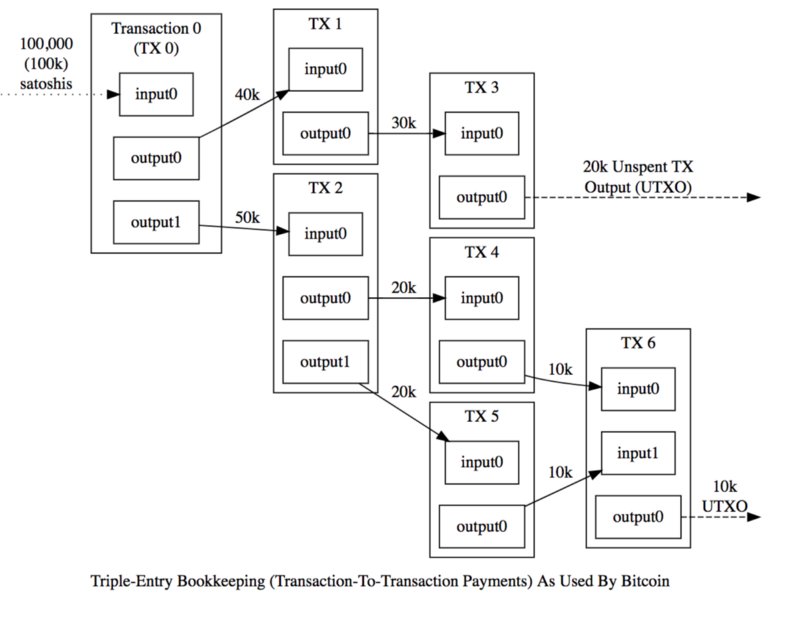
\includegraphics[scale = 0.5]{utxo}

Existem várias vantagens e desvantagens desse tipo de estrutura de dados. Uma das desvantagens é que é bastante custoso verificar o saldo da conta, pois é necessário calcular todas as transações vinculadas a conta. Outra desvantagem é que esse modelo é mais complexo.

Já suas vantagens são outras. Esse tipo de estrutura de dados permite escalabilidade, pois o paralelismo é permitido. Já que uma mesma conta pode por exemplo gastar várias transações não gastas ao mesmo tempo. Outra vantagem seria a privacidade, pois um mesmo usuário pode criar uma conta nova por transação.

No paper de Anton Setzer, a modelagem da estrutura de dados do UTXO está quase terminada.

\section{Blockchain em Agda}

A estrutura de dados blockchain significa cadeia de blocos. Existem dois tipos de blocos, o primeiro bloco (genesis block) e os outros. Cada bloco, possui um link para o bloco anterior (exceto o primeiro). Esse link é o hash do bloco anterior. Dessa forma, é possível sempre garantir a ordem dos blocos. Cada bloco armazena transações, o hash do bloco anterior, o nounce e o seu próprio hash. Cada bloco precisa ser minerado, ou seja, o minerador precisa calcular o valor do nounce (que é preciso de muito poder computacional).

Dessa forma, foi adicionado no código de Agda, a especificação de que o bloco deve conter o hash do bloco anterior, usando tipos dependentes. E a especificação do hash do bloco.

\ExecuteMetaData[latex/Code.tex]{blockchain}

\section{Metodologia}

O trabalho está sendo programado na linguagem Agda, provador de teoremas. 

Para controle de versão, é utilizado o Git com Github.
Com o Github, é possível fazer integração contínua com Travis CI ou Hydra.
Ou seja, a cada novo commit, é instanciada uma máquina virtual para compilar o projeto todo.

O gerenciador de pacotes utilizado é o Nix. É um gerenciador de pacotes funcional. 
Ou seja, é feito de forma descritiva como será compilado o projeto.

Para compilação dos slides e da dissertação, é utilizado Latex e latexmk e todo o resto acima.
Todo código colocado nos slides e na dissertação são compilados antes. Dessa forma, não existe perigo de haver algum código que não funcione.

O trabalho será feito usando a metodologia do livro Type Driven Development. Ou seja, enquanto a criptomoeda for programada, o seu tipo será refinado conforme as necessidades. Caso algo ainda não seja provado com os tipos, uma prova formal será adicionada posteriormente.

\newpage
\section{Agradecimento}

Agradeço o professor Flávio por me auxiliar em todas as minhas dúvidas sobre bitcoin e me ajudar na escrita da minha dissertação. 
Agradeço aos livros e papers que encontrei, pois muitas dúvidas já estavam solucionadas por lá.

\newpage
 
\begin{thebibliography}{111}

\bibitem{Agda Compiler}
    Andreas Abel, 
    {\it Stephan Adelsberger, and Anton Setzer. ooAgda. Agda Library, 2016. 
    \url{https://github.com/agda/ooAgda}}
    
\bibitem{Agda Documentation}
    Andreas Abel, Stephan Adelsberger, and Anton Setzer. ooAgda. Agda Library, 2016. 
    \url{https://github.com/agda/ooAgda}

\bibitem{Agda Wiki}
    Agda Wiki.  The Agda Wiki, 2017.  
    \url{http://wiki.portal.chalmers.se/agda/pmwiki.php}
    
\bibitem{Bitcoin whitepaper}
    Satoshi Nakamoto.  
    {\it Bitcoin:  A peer-to-peer electronic cash system, 1 November 2008.Announced on the cryptography mailing list. \url{http://www.bitcoin.org/bitcoin.pdf}}

\bibitem{Bitcoin whitepaper2}
    Satoshi Nakamoto.  
    {\it Satoshi Nakamoto.  Bitcoin:  A peer-to-peer electronic cash system, 1 November 2008.Announced on the cryptography mailing list. \url{http://www.bitcoin.org/bitcoin.pdf}}

\bibitem{Modelling Bitcoin in Agda}
Anton Setzer.  
{\it ept. of Computer Science, Swansea University, Singleton Park, Swansea SA28PP, UK}

\end{thebibliography}
\end{document}
